% Options for packages loaded elsewhere
\PassOptionsToPackage{unicode}{hyperref}
\PassOptionsToPackage{hyphens}{url}
\PassOptionsToPackage{dvipsnames,svgnames*,x11names*}{xcolor}
%
\documentclass[
]{article}
\usepackage{amsmath,amssymb}
\usepackage{lmodern}
\usepackage{ifxetex,ifluatex}
\ifnum 0\ifxetex 1\fi\ifluatex 1\fi=0 % if pdftex
  \usepackage[T1]{fontenc}
  \usepackage[utf8]{inputenc}
  \usepackage{textcomp} % provide euro and other symbols
\else % if luatex or xetex
  \usepackage{unicode-math}
  \defaultfontfeatures{Scale=MatchLowercase}
  \defaultfontfeatures[\rmfamily]{Ligatures=TeX,Scale=1}
\fi
% Use upquote if available, for straight quotes in verbatim environments
\IfFileExists{upquote.sty}{\usepackage{upquote}}{}
\IfFileExists{microtype.sty}{% use microtype if available
  \usepackage[]{microtype}
  \UseMicrotypeSet[protrusion]{basicmath} % disable protrusion for tt fonts
}{}
\makeatletter
\@ifundefined{KOMAClassName}{% if non-KOMA class
  \IfFileExists{parskip.sty}{%
    \usepackage{parskip}
  }{% else
    \setlength{\parindent}{0pt}
    \setlength{\parskip}{6pt plus 2pt minus 1pt}}
}{% if KOMA class
  \KOMAoptions{parskip=half}}
\makeatother
\usepackage{xcolor}
\IfFileExists{xurl.sty}{\usepackage{xurl}}{} % add URL line breaks if available
\IfFileExists{bookmark.sty}{\usepackage{bookmark}}{\usepackage{hyperref}}
\hypersetup{
  pdftitle={Meeting2},
  pdfauthor={Kuan Liu},
  colorlinks=true,
  linkcolor=Maroon,
  filecolor=Maroon,
  citecolor=Blue,
  urlcolor=blue,
  pdfcreator={LaTeX via pandoc}}
\urlstyle{same} % disable monospaced font for URLs
\usepackage[margin=1in]{geometry}
\usepackage{color}
\usepackage{fancyvrb}
\newcommand{\VerbBar}{|}
\newcommand{\VERB}{\Verb[commandchars=\\\{\}]}
\DefineVerbatimEnvironment{Highlighting}{Verbatim}{commandchars=\\\{\}}
% Add ',fontsize=\small' for more characters per line
\usepackage{framed}
\definecolor{shadecolor}{RGB}{248,248,248}
\newenvironment{Shaded}{\begin{snugshade}}{\end{snugshade}}
\newcommand{\AlertTok}[1]{\textcolor[rgb]{0.94,0.16,0.16}{#1}}
\newcommand{\AnnotationTok}[1]{\textcolor[rgb]{0.56,0.35,0.01}{\textbf{\textit{#1}}}}
\newcommand{\AttributeTok}[1]{\textcolor[rgb]{0.77,0.63,0.00}{#1}}
\newcommand{\BaseNTok}[1]{\textcolor[rgb]{0.00,0.00,0.81}{#1}}
\newcommand{\BuiltInTok}[1]{#1}
\newcommand{\CharTok}[1]{\textcolor[rgb]{0.31,0.60,0.02}{#1}}
\newcommand{\CommentTok}[1]{\textcolor[rgb]{0.56,0.35,0.01}{\textit{#1}}}
\newcommand{\CommentVarTok}[1]{\textcolor[rgb]{0.56,0.35,0.01}{\textbf{\textit{#1}}}}
\newcommand{\ConstantTok}[1]{\textcolor[rgb]{0.00,0.00,0.00}{#1}}
\newcommand{\ControlFlowTok}[1]{\textcolor[rgb]{0.13,0.29,0.53}{\textbf{#1}}}
\newcommand{\DataTypeTok}[1]{\textcolor[rgb]{0.13,0.29,0.53}{#1}}
\newcommand{\DecValTok}[1]{\textcolor[rgb]{0.00,0.00,0.81}{#1}}
\newcommand{\DocumentationTok}[1]{\textcolor[rgb]{0.56,0.35,0.01}{\textbf{\textit{#1}}}}
\newcommand{\ErrorTok}[1]{\textcolor[rgb]{0.64,0.00,0.00}{\textbf{#1}}}
\newcommand{\ExtensionTok}[1]{#1}
\newcommand{\FloatTok}[1]{\textcolor[rgb]{0.00,0.00,0.81}{#1}}
\newcommand{\FunctionTok}[1]{\textcolor[rgb]{0.00,0.00,0.00}{#1}}
\newcommand{\ImportTok}[1]{#1}
\newcommand{\InformationTok}[1]{\textcolor[rgb]{0.56,0.35,0.01}{\textbf{\textit{#1}}}}
\newcommand{\KeywordTok}[1]{\textcolor[rgb]{0.13,0.29,0.53}{\textbf{#1}}}
\newcommand{\NormalTok}[1]{#1}
\newcommand{\OperatorTok}[1]{\textcolor[rgb]{0.81,0.36,0.00}{\textbf{#1}}}
\newcommand{\OtherTok}[1]{\textcolor[rgb]{0.56,0.35,0.01}{#1}}
\newcommand{\PreprocessorTok}[1]{\textcolor[rgb]{0.56,0.35,0.01}{\textit{#1}}}
\newcommand{\RegionMarkerTok}[1]{#1}
\newcommand{\SpecialCharTok}[1]{\textcolor[rgb]{0.00,0.00,0.00}{#1}}
\newcommand{\SpecialStringTok}[1]{\textcolor[rgb]{0.31,0.60,0.02}{#1}}
\newcommand{\StringTok}[1]{\textcolor[rgb]{0.31,0.60,0.02}{#1}}
\newcommand{\VariableTok}[1]{\textcolor[rgb]{0.00,0.00,0.00}{#1}}
\newcommand{\VerbatimStringTok}[1]{\textcolor[rgb]{0.31,0.60,0.02}{#1}}
\newcommand{\WarningTok}[1]{\textcolor[rgb]{0.56,0.35,0.01}{\textbf{\textit{#1}}}}
\usepackage{graphicx}
\makeatletter
\def\maxwidth{\ifdim\Gin@nat@width>\linewidth\linewidth\else\Gin@nat@width\fi}
\def\maxheight{\ifdim\Gin@nat@height>\textheight\textheight\else\Gin@nat@height\fi}
\makeatother
% Scale images if necessary, so that they will not overflow the page
% margins by default, and it is still possible to overwrite the defaults
% using explicit options in \includegraphics[width, height, ...]{}
\setkeys{Gin}{width=\maxwidth,height=\maxheight,keepaspectratio}
% Set default figure placement to htbp
\makeatletter
\def\fps@figure{htbp}
\makeatother
\setlength{\emergencystretch}{3em} % prevent overfull lines
\providecommand{\tightlist}{%
  \setlength{\itemsep}{0pt}\setlength{\parskip}{0pt}}
\setcounter{secnumdepth}{-\maxdimen} % remove section numbering
\ifluatex
  \usepackage{selnolig}  % disable illegal ligatures
\fi

\title{Meeting2}
\author{Kuan Liu}
\date{Aug 03 2021}

\begin{document}
\maketitle

\hypertarget{chapter-3-phase-i}{%
\section{Chapter 3 Phase I}\label{chapter-3-phase-i}}

Generally speaking the Objectives of Phase I study is safety and dosage.
This chapter focuses on Phase I methods to identify the maximum
tolerated dose (MTD). Key elements of Phase I studies including,

\begin{itemize}
\item
  \begin{enumerate}
  \def\labelenumi{(\arabic{enumi})}
  \setcounter{enumi}{-1}
  \tightlist
  \item
    study population (healthy volunteers or people with disease)
  \end{enumerate}
\item
  \begin{enumerate}
  \def\labelenumi{(\alph{enumi})}
  \tightlist
  \item
    starting dose (e.g.~\(LD_{10}\))
  \end{enumerate}
\item
  \begin{enumerate}
  \def\labelenumi{(\alph{enumi})}
  \setcounter{enumi}{1}
  \tightlist
  \item
    toxicity profile and dose-limiting toxicity (DLT)
  \end{enumerate}
\item
  \begin{enumerate}
  \def\labelenumi{(\alph{enumi})}
  \setcounter{enumi}{2}
  \tightlist
  \item
    target toxicity level (TTL)
  \end{enumerate}
\item
  \begin{enumerate}
  \def\labelenumi{(\alph{enumi})}
  \setcounter{enumi}{3}
  \tightlist
  \item
    dose escalation scheme (dose increment, dose assignment and cohort
    size)
  \end{enumerate}
\end{itemize}

\hypertarget{rule-based-design-for-determing-maximum-tolerated-dose-mtd}{%
\subsection{3.1 Rule-based design for determing maximum tolerated dose
(MTD)}\label{rule-based-design-for-determing-maximum-tolerated-dose-mtd}}

\hypertarget{design-storer-eb-1989}{%
\subsubsection{3+3 design (Storer EB,
1989)}\label{design-storer-eb-1989}}

\begin{itemize}
\tightlist
\item
  widely used, implementation does not require a computer
\item
  simplicity: dose escalation and de-escalation decisions are based on a
  set of prespecified rules
\item
  Example 3.2, page 90, 3+3 can be inefficient with low starting dose
  and small to moderate increment.
\end{itemize}

\hypertarget{pharmacologically-guided-dose-escalation}{%
\subsubsection{Pharmacologically guided dose
escalation}\label{pharmacologically-guided-dose-escalation}}

\begin{itemize}
\tightlist
\item
  considered more efficient then 3+3, but doesn't work for all agents
  and there are challenges in getting timely pharmacokinetic results.
\end{itemize}

\hypertarget{accelerated-titration-designs-and-other-rule-based-designs}{%
\subsubsection{Accelerated titration designs and other rule-based
designs}\label{accelerated-titration-designs-and-other-rule-based-designs}}

\begin{itemize}
\tightlist
\item
  variation of 3+3, allow intrapatient dose escalation - reduce number
  of patients
\item
  drawbacks: mask of efficacy and toxicity (delayed)
\end{itemize}

\hypertarget{other-rule-based-designs}{%
\subsubsection{Other rule-based
designs}\label{other-rule-based-designs}}

Newest one, the i3+3 design
\href{https://www.tandfonline.com/doi/abs/10.1080/10543406.2019.1636811?journalCode=lbps20}{(Liu
M, 2020)}. Set of dose \(d=1, \ldots, D\) and pre-specified i) target
toxicity rate, \(p_T\) (e.g., \(p_T=0.3\)) and the equivalence interval
(EI), mathematically as \([p_T - \epsilon_1, p_T + \epsilon_2]\) (e.g.,
{[}0.25, 0.35{]}). EI provides a range around \(p_T\) so that doses with
toxicity probabilities inside EI are considered as MTD - allows some
variabilities.

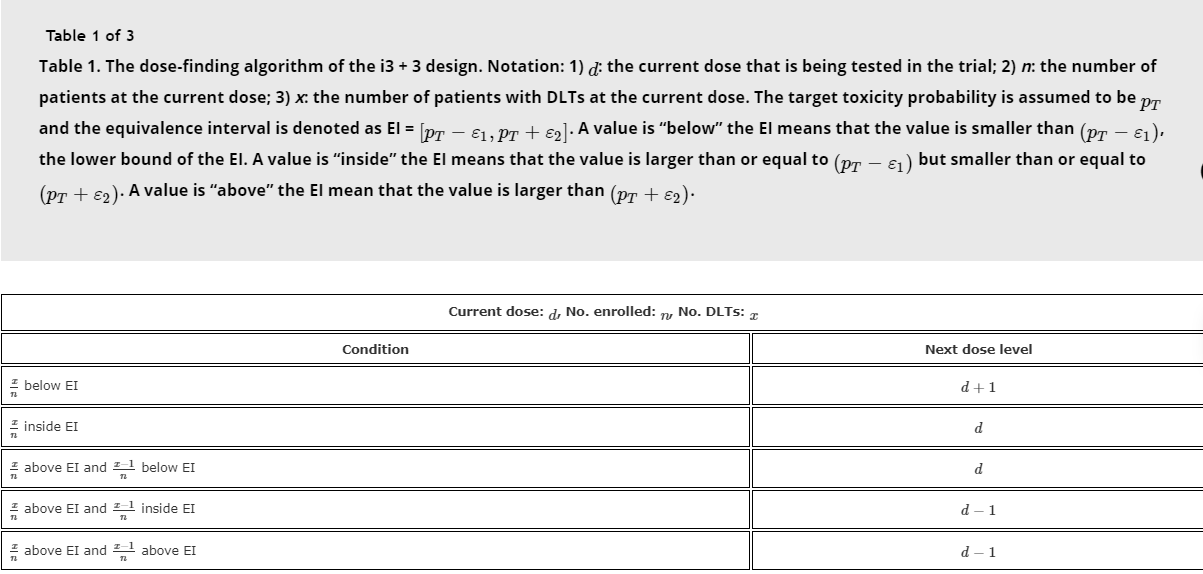
\includegraphics[width=1.1\textwidth,height=\textheight]{Figurei33.PNG}

\hypertarget{summary}{%
\subsubsection{Summary}\label{summary}}

simple but potentially inefficient.

\hypertarget{model-based-designs}{%
\subsection{3.2 Model-based designs}\label{model-based-designs}}

These designs assume a monotonic dose-response relationship with defined
dose-toxicity curve and target toxicity level. Works well under Bayesian
framework.

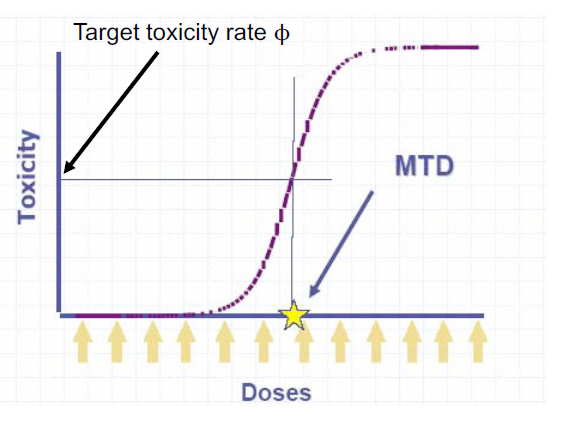
\includegraphics[width=0.55\textwidth,height=\textheight]{Figure3.1_sub.PNG}

\hypertarget{continual-reassessment-method-crm}{%
\subsubsection{Continual reassessment method
(CRM)}\label{continual-reassessment-method-crm}}

\begin{itemize}
\item
  common model for dose-toxicity curve: hyperbolic tangent, logistic,
  power. Model is updated based on accrued data (Bayesian adaptation)
\item
  more likely to identify correct MTD comparing to 3+3
\item
  Not well-accepted in original format due to safety considerations , if
  pre-specified model were incorrect.
\item
  online shiny app,
  \url{https://trialdesign.org/one-page-shell.html\#BMACRM}
\end{itemize}

\hypertarget{escalation-with-overdose-control-ewoc}{%
\subsubsection{Escalation with overdose control
(EWOC)}\label{escalation-with-overdose-control-ewoc}}

\begin{itemize}
\tightlist
\item
  same as CRM except the way it selects each successive new dose
\item
  unlike CRM that select the new dose using the posterior mode or mean,
  EWOC use the feasibility bound. A feasibility bound \(\alpha < 0.5\)
  corresponds to placing a higher penalty on overdosing than on
  underdosing.
\end{itemize}

\begin{Shaded}
\begin{Highlighting}[]
\FunctionTok{library}\NormalTok{(R2jags)}
\FunctionTok{library}\NormalTok{(runjags)}

\NormalTok{filename }\OtherTok{\textless{}{-}} \StringTok{"BUGSmodel.txt"}
\FunctionTok{cat}\NormalTok{(}\StringTok{"}
\StringTok{model\{}
\StringTok{    for (i in 1:N)\{}
\StringTok{\# Likelihood}
\StringTok{      Y[i]\textasciitilde{}dbern(p[i])}
\StringTok{      logit(p[i])\textless{}{-} (1/(gamma {-} Xmin))*(gamma*logit(rho0) }
\StringTok{      {-} Xmin*logit(theta)+(logit(theta){-}logit(rho0))*X[i])}
\StringTok{    \}  \#  end of for loop}
\StringTok{\# Priors}
\StringTok{    gamma \textasciitilde{} dunif(Xmin, Xmax)}
\StringTok{    rho0 \textasciitilde{} dunif(0,theta)}
\StringTok{  \}  \#  end of BUGS code}

\StringTok{"}\NormalTok{,}\AttributeTok{file=}\NormalTok{filename}
\NormalTok{)}

\CommentTok{\# Data (1st patient 140, no tox):}
\NormalTok{data1}\OtherTok{\textless{}{-}}\FunctionTok{list}\NormalTok{(}\AttributeTok{Y=}\FunctionTok{c}\NormalTok{(}\DecValTok{0}\NormalTok{), }\AttributeTok{X=}\FunctionTok{c}\NormalTok{(}\DecValTok{140}\NormalTok{), }\AttributeTok{Xmin=}\DecValTok{140}\NormalTok{, }\AttributeTok{Xmax =}\DecValTok{425}\NormalTok{, }\AttributeTok{theta=}\FloatTok{0.333}\NormalTok{, }\AttributeTok{N=}\DecValTok{1}\NormalTok{)}

\CommentTok{\# Data (1st patient 140, no tox; 2nd patient 210, no tox):}
\NormalTok{data2}\OtherTok{\textless{}{-}}\FunctionTok{list}\NormalTok{(}\AttributeTok{Y=}\FunctionTok{c}\NormalTok{(}\DecValTok{0}\NormalTok{,}\DecValTok{0}\NormalTok{), }\AttributeTok{X=}\FunctionTok{c}\NormalTok{(}\DecValTok{140}\NormalTok{,}\DecValTok{210}\NormalTok{), }\AttributeTok{Xmin=}\DecValTok{140}\NormalTok{, }\AttributeTok{Xmax=}\DecValTok{425}\NormalTok{, }\AttributeTok{theta=}\FloatTok{0.333}\NormalTok{, }\AttributeTok{N=}\DecValTok{2}\NormalTok{)   }
    
\CommentTok{\# Data (1st patient 140, no tox; 2nd patient 210, tox):}
\NormalTok{data3}\OtherTok{\textless{}{-}}\FunctionTok{list}\NormalTok{(}\AttributeTok{Y=}\FunctionTok{c}\NormalTok{(}\DecValTok{0}\NormalTok{,}\DecValTok{1}\NormalTok{), }\AttributeTok{X=}\FunctionTok{c}\NormalTok{(}\DecValTok{140}\NormalTok{,}\DecValTok{210}\NormalTok{), }\AttributeTok{Xmin=}\DecValTok{140}\NormalTok{, }\AttributeTok{Xmax=}\DecValTok{425}\NormalTok{, }\AttributeTok{theta=}\FloatTok{0.333}\NormalTok{, }\AttributeTok{N=}\DecValTok{2}\NormalTok{)   }
    
\CommentTok{\# Data (1st patient 140, no tox; 2nd patient 210, no tox;}
\CommentTok{\#   3rd patient 300, no response yet):}
\NormalTok{data4}\OtherTok{\textless{}{-}}\FunctionTok{list}\NormalTok{(}\AttributeTok{Y=}\FunctionTok{c}\NormalTok{(}\DecValTok{0}\NormalTok{,}\DecValTok{0}\NormalTok{,}\ConstantTok{NA}\NormalTok{),}\AttributeTok{X=}\FunctionTok{c}\NormalTok{(}\DecValTok{140}\NormalTok{,}\DecValTok{210}\NormalTok{,}\DecValTok{300}\NormalTok{),}\AttributeTok{Xmin=}\DecValTok{140}\NormalTok{,}\AttributeTok{Xmax=}\DecValTok{425}\NormalTok{,}\AttributeTok{theta=}\FloatTok{0.333}\NormalTok{,}\AttributeTok{N=}\DecValTok{3}\NormalTok{) }
    
\CommentTok{\#Inits:}
\NormalTok{init}\OtherTok{\textless{}{-}}\FunctionTok{list}\NormalTok{(}\FunctionTok{list}\NormalTok{(}\AttributeTok{rho0=}\FloatTok{0.05}\NormalTok{, }\AttributeTok{gamma=}\DecValTok{160}\NormalTok{),}\FunctionTok{list}\NormalTok{(}\AttributeTok{rho0=}\FloatTok{0.05}\NormalTok{, }\AttributeTok{gamma=}\DecValTok{160}\NormalTok{))}

\CommentTok{\#First patient;}
\NormalTok{jags.fit }\OtherTok{\textless{}{-}} \FunctionTok{jags}\NormalTok{(}\AttributeTok{data=}\NormalTok{data1,}\AttributeTok{inits=}\NormalTok{init,}\AttributeTok{parameters.to.save=}\FunctionTok{c}\NormalTok{(}\StringTok{"rho0"}\NormalTok{,}\StringTok{"gamma"}\NormalTok{),}
         \AttributeTok{jags.seed =} \DecValTok{100}\NormalTok{, }\AttributeTok{n.iter=}\DecValTok{11000}\NormalTok{, }\AttributeTok{model.file=}\StringTok{"BUGSmodel.txt"}\NormalTok{,}\AttributeTok{n.chains =} \DecValTok{2}\NormalTok{,}\AttributeTok{n.burnin =} \DecValTok{1000}\NormalTok{)}
\end{Highlighting}
\end{Shaded}

\begin{verbatim}
## Compiling model graph
##    Resolving undeclared variables
##    Allocating nodes
## Graph information:
##    Observed stochastic nodes: 1
##    Unobserved stochastic nodes: 2
##    Total graph size: 22
## 
## Initializing model
\end{verbatim}

\begin{Shaded}
\begin{Highlighting}[]
\NormalTok{jagsfit.mcmc}\OtherTok{\textless{}{-}} \FunctionTok{as.mcmc}\NormalTok{(jags.fit)}
\FunctionTok{summary}\NormalTok{(jagsfit.mcmc)}
\end{Highlighting}
\end{Shaded}

\begin{verbatim}
## 
## Iterations = 1001:10991
## Thinning interval = 10 
## Number of chains = 2 
## Sample size per chain = 1000 
## 
## 1. Empirical mean and standard deviation for each variable,
##    plus standard error of the mean:
## 
##              Mean       SD Naive SE Time-series SE
## deviance   0.3474  0.22610 0.005056       0.005106
## gamma    285.3061 82.29270 1.840121       1.918351
## rho0       0.1541  0.09389 0.002099       0.002118
## 
## 2. Quantiles for each variable:
## 
##               2.5%       25%      50%      75%    97.5%
## deviance 1.226e-02   0.15068   0.3226   0.5291   0.7753
## gamma    1.466e+02 214.95002 284.4832 356.7328 419.4510
## rho0     6.113e-03   0.07257   0.1489   0.2324   0.3214
\end{verbatim}

\begin{Shaded}
\begin{Highlighting}[]
\CommentTok{\#Second patient;}
\NormalTok{jags.fit }\OtherTok{\textless{}{-}} \FunctionTok{jags}\NormalTok{(}\AttributeTok{data=}\NormalTok{data2,}\AttributeTok{inits=}\NormalTok{init,}\AttributeTok{parameters.to.save=}\FunctionTok{c}\NormalTok{(}\StringTok{"rho0"}\NormalTok{,}\StringTok{"gamma"}\NormalTok{),}
         \AttributeTok{jags.seed =} \DecValTok{100}\NormalTok{, }\AttributeTok{n.iter=}\DecValTok{11000}\NormalTok{, }\AttributeTok{model.file=}\StringTok{"BUGSmodel.txt"}\NormalTok{,}\AttributeTok{n.chains =} \DecValTok{2}\NormalTok{,}\AttributeTok{n.burnin =} \DecValTok{1000}\NormalTok{)}
\end{Highlighting}
\end{Shaded}

\begin{verbatim}
## Compiling model graph
##    Resolving undeclared variables
##    Allocating nodes
## Graph information:
##    Observed stochastic nodes: 2
##    Unobserved stochastic nodes: 2
##    Total graph size: 28
## 
## Initializing model
\end{verbatim}

\begin{Shaded}
\begin{Highlighting}[]
\NormalTok{jagsfit.mcmc}\OtherTok{\textless{}{-}} \FunctionTok{as.mcmc}\NormalTok{(jags.fit)}
\FunctionTok{summary}\NormalTok{(jagsfit.mcmc)}
\end{Highlighting}
\end{Shaded}

\begin{verbatim}
## 
## Iterations = 1001:10991
## Thinning interval = 10 
## Number of chains = 2 
## Sample size per chain = 1000 
## 
## 1. Empirical mean and standard deviation for each variable,
##    plus standard error of the mean:
## 
##              Mean      SD Naive SE Time-series SE
## deviance   0.9380  0.5703 0.012751       0.012309
## gamma    302.7255 73.6253 1.646311       1.646506
## rho0       0.1552  0.0955 0.002135       0.002136
## 
## 2. Quantiles for each variable:
## 
##               2.5%       25%      50%      75%    97.5%
## deviance 1.128e-01   0.51521   0.8942   1.3098   1.9733
## gamma    1.698e+02 241.47122 305.7341 364.3646 420.4591
## rho0     8.251e-03   0.07285   0.1481   0.2353   0.3222
\end{verbatim}

\hypertarget{time-to-event-monitoring-tite-crm}{%
\subsubsection{Time-to-event monitoring
(TITE-CRM)}\label{time-to-event-monitoring-tite-crm}}

\hypertarget{quick-summary-on-crm-based-approaches}{%
\subsubsection{Quick Summary on CRM based
approaches}\label{quick-summary-on-crm-based-approaches}}

Pros:

\begin{itemize}
\tightlist
\item
  Solid statistical foundation
\item
  Flexible and efficient
\item
  Better performance than rule-based
\end{itemize}

Cons:

\begin{itemize}
\tightlist
\item
  Performance can be compromised when the model is misspecified
\item
  Need specialized expertise to select prior and model
\item
  Work like a black box, challenging to communicate with
  non-statisticians
\end{itemize}

\hypertarget{toxicity-intervals-and-ordinal-toxicity-intervals}{%
\subsubsection{Toxicity intervals and Ordinal toxicity
intervals}\label{toxicity-intervals-and-ordinal-toxicity-intervals}}

\begin{itemize}
\tightlist
\item
  allow the use of a range of acceptable toxicity levels
\item
  this methods is introduced to incorporate uncertainty in estimating
  mean toxicities
\item
  does not skip does and stops early for excessive toxicity if the
  lowest does is found to be excessively toxic
\end{itemize}

\hypertarget{efficacy-versus-toxicity}{%
\subsection{3.3 Efficacy versus
toxicity}\label{efficacy-versus-toxicity}}

\begin{itemize}
\tightlist
\item
  dose finding incorporating both efficacy and toxicity endpoints
\item
  Use for Phase I/II design, seamless phase I and II
\item
  \(EffTox\),
  \href{https://biostatistics.mdanderson.org/SoftwareDownload/SingleSoftware/Index/2}{link
  to software}, \href{https://www.johndcook.com/efftox.pdf}{link to
  paper}
\end{itemize}

Pair of binary outcomes, \((Y_E, Y_T)\) follow with marginal probability
in logit form as

\[logit(\pi_T) = \mu_T + \beta_T x\]
\[logit(\pi_E) = \mu_E + \beta_{E,1} x + \beta_{E,2} x^2\] where x is
the dosing variable. The bivariate joint likelihood
\(P(Y_E=a, Y_T=b \mid \theta)\) captures the dependency between the two
outcomes, where \(a \in \{0,1\}\), \(b \in \{0,1\}\) and \(\theta\)
presents the vector of parameters.

At each dose update decision, the dose \(x\) is acceptable if
\[ P \{ \pi_{E} (x, \theta) \leq \pi_{\bar{E}} (x, \theta) \mid D_n \} > p_E\]
and

\[P \{ \pi_{T} (x, \theta) < \pi_{\bar{T}} (x, \theta) \mid D_n \} < p_T\]
\(p_E\) and \(p_T\) are pre-defined gatekeepers for meeting minimum
efficacy and maximum toxicity. Larger \(p_E\) more likely to exclude low
efficacy doses and larger \(p_T\) more likely to exclude excessive
toxicity doses.

The utility (desirability measure, the larger the better) of dose x with
\(\pi_E(x, \theta)\) and \(\pi_T(x, \theta)\) - which is used to assess
efficacy-toxicity trade-off is

\[ u(\pi_E, \pi_T) = 1 - \Big[ (\frac{1-\pi_E}{1-\pi_E^{*}})^p + (\frac{\pi_T}{\pi_T^{*}})^p \Big]^{\frac{1}{p}}\]
where \(\pi_E^{*}\) represents the smallest acceptable efficacy response
rate and \(\pi_T^{*}\) represents the highest acceptable toxicity level.

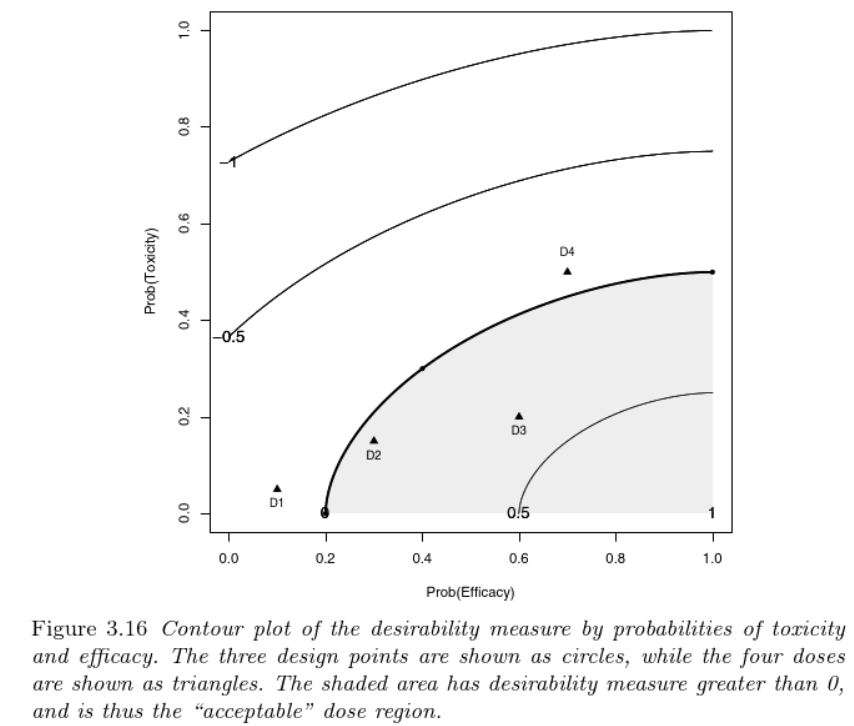
\includegraphics[width=0.8\textwidth,height=\textheight]{Figure3.16.PNG}

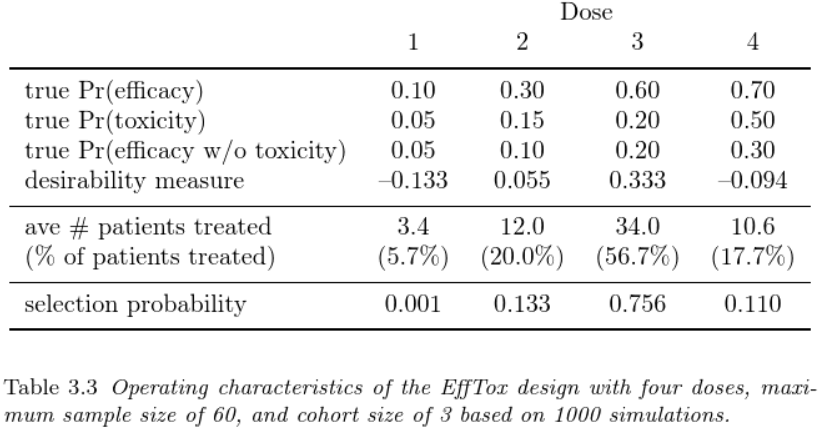
\includegraphics[width=0.7\textwidth,height=\textheight]{Table3.3.PNG}

\hypertarget{combination-therapy}{%
\subsection{3.4 Combination therapy}\label{combination-therapy}}

\begin{itemize}
\item
  mathematically similar to efficacy and toxicity joint modelling, now
  we joint model two or more toxicity models for each combination
  therapy
\item
  Gumbel model, good but might be sensible to changes of the algorithm
\item
  Bivariate CRM
\item
  Combination therapy with bivariate response (toxicity and efficacy)
\item
  Bivariate logistic model
\end{itemize}

\hypertarget{additional-readings}{%
\subsection{Additional Readings}\label{additional-readings}}

\begin{enumerate}
\def\labelenumi{\arabic{enumi}.}
\setcounter{enumi}{-1}
\tightlist
\item
  Review of current Phase I methods (recommanded),
  \url{https://clincancerres.aacrjournals.org/content/24/18/4357}
\item
  Phase 0 (a proof of principle trial involving small number of
  patients), \url{https://www.ncbi.nlm.nih.gov/pmc/articles/PMC3902019/}
\item
  Seamless early-phase designs in oncology,
  \url{https://academic.oup.com/jnci/article/111/2/118/5245491}
\item
  Model-assisted phase I design, Bayesian optimal interval design (BOIN)
  \href{https://doi.org/10.1111/rssc.12089}{(Liu and Yuan, 2015)}
\end{enumerate}

\end{document}
